
\chapter{Referencial Teórico}

\section{Pessoas como Sensores Voluntários}
Para a compreensão da utilização de pessoas como sensores vê-se necessário o entendimento dos conceitos de User-generated content (UGC), World Wide Web 2.0 (WEB 2.0), Neogeografia, Inteligência Coletiva, e Volunteered Geographic Information (VGI), os quais serão apresentados a seguir. 

UGC (User-Genereted Content – Conteúdo Gerado pelo Usuário) segundo \cite{santos_avaliacao_2016}, se refere a ação dos usuários compartilharem suas experiências e com isso produzir um grande volume de informações. Um dos mais populares exemplos é a Wikipédia, uma plataforma colaborativa que contém mais de 1.000,000 artigos em português e 6,292 usuários ativos, este número vem crescendo constantemente \cite{Wikipedia2018}.

A WEB 2.0 representa uma maneira diferente de interagir com a internet, pois oferece maior autonomia para o usuário no sistema, na medida em que possibilita a criação de conteúdo e a avaliação daquilo que consome. \citeonline [p.~2]{Primo2007} afirma que Web 2.0 é a uma nova geração de serviços na rede, identificada  por suas diversas formas de produção contributiva e partilhamento de informações online. Plataformas como Twitter e Youtube, com centenas de milhões de usuários, tem se adaptando para melhor atender seu público por meio da implementação de recursos que facilitam tanto a criação quanto à visualização de conteúdo. 

O termo Neogeografia (nova geografia) para \citeonline[p.~228]{machado_os_2014} Machado (2014), é um fenômeno social que gira em torno do crescimento em massa dos mapas virtuais, e ao facilitamento de uso de tecnologias com ferramentas para posicionamento como o GPS.

Para \citeonline[p.~28]{Levy2007}, inteligência coletiva é "uma inteligência distribuída por toda parte, incessantemente valorizada, coordenada em tempo real, que resulta em uma mobilização efetiva das competências".

De acordo com \apudonline[p.~10]{Goodchild2007}{miranda_uma_2010}, VGI é uma expressão usado para definir a informações geográficas que são produzidas através de usuários, que funde elementos da Web 2.0, Inteligência Coletiva e Neogeografia e que atinge as necessidades da indústria, do governo e das comunidades de redes sociais. O conjunto de dados e as informações deles decorrentes são, por meio de plataformas de inteligência coletiva, avaliados, validados e consolidados pelos usuários, inclusive aqueles que geraram a informação.

\section{O Sistema WEB Cidadão do Vale}
Conforme exposto, a plataforma Cidadão do Vale foi implementada no município de Almenara-MG como alternativa a informação de problemas urbanos e de gestão municipal. O sistema Cidadão do Vale foi disponibilizado de forma pública sob o domínio \url{www.cidadaodovale.xyz}, em funcionamento completo que inclui a visualização e contribuição de dados do sistema. Na Figura 3 é apresentada a página inicial, onde se encontra as colaborações georreferenciadas cadastradas no sistema em 3 de agosto de 2018. A Figura 4 corresponde a tela de cadastro de usuário, e as Figuras 5 e 6 correspondem aos mapas de calor referentes às contribuições sobre limpeza urbana e vias públicas em 3 de agosto de 2018.

% PÁGINA INICIAL
\begin{figure}[H]
	\centering
	\caption{Página inicial da plataforma Cidadão do Vale.}
	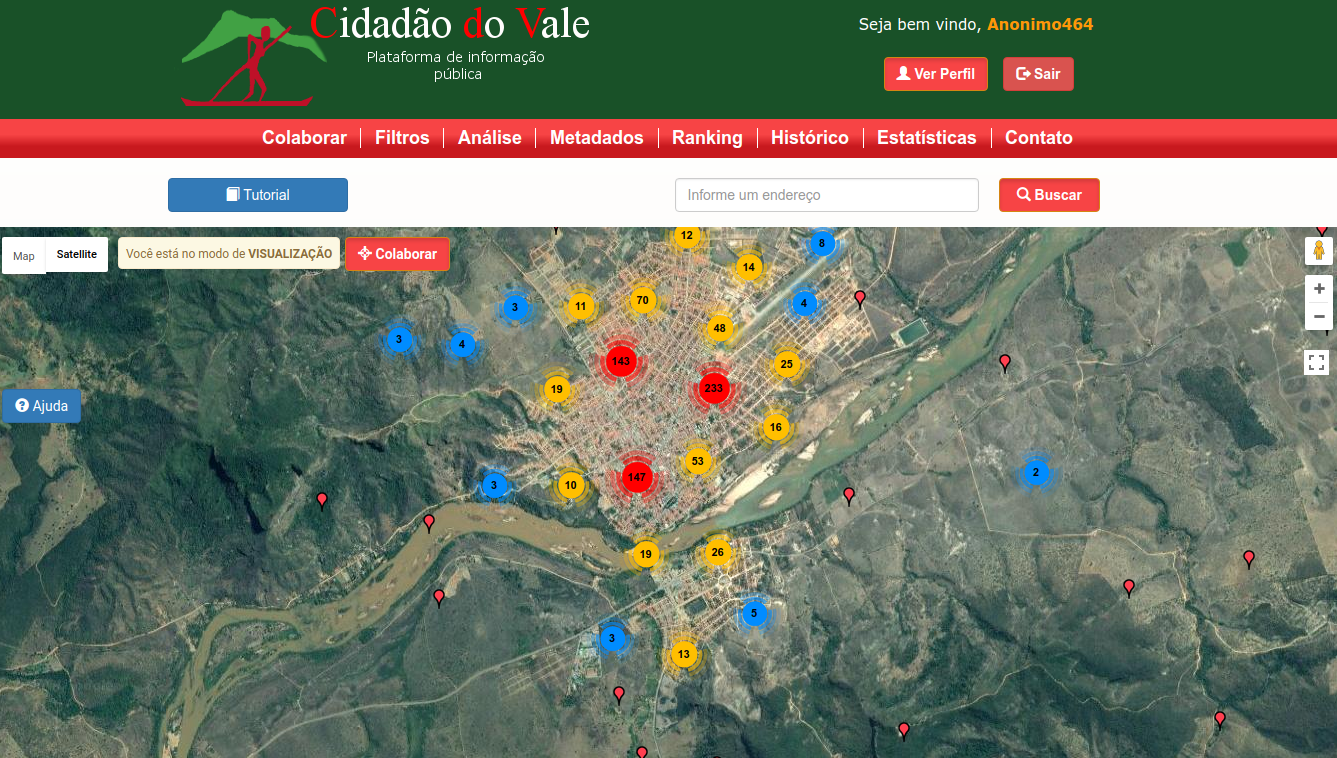
\includegraphics[width=0.6\linewidth]{Imagens/01}
	\legend{Fonte:\url{http://www.cidadaodovale.xyz/inicio.php}}
\end{figure}

% CADASTRO
\begin{figure}[H]
	\centering
	\caption{Página de cadastro do sistema Cidadão do Vale}	
	
\includegraphics[width=0.6\linewidth]{Imagens/02}
	\legend{Fonte:\url{http://www.cidadaodovale.xyz/registro.php}}
\end{figure}

% LIMPEZA URBANA
\begin{figure}[H]
	\centering
	\caption{Densidade Kernel das contribuições sobre limpeza urbana.}
	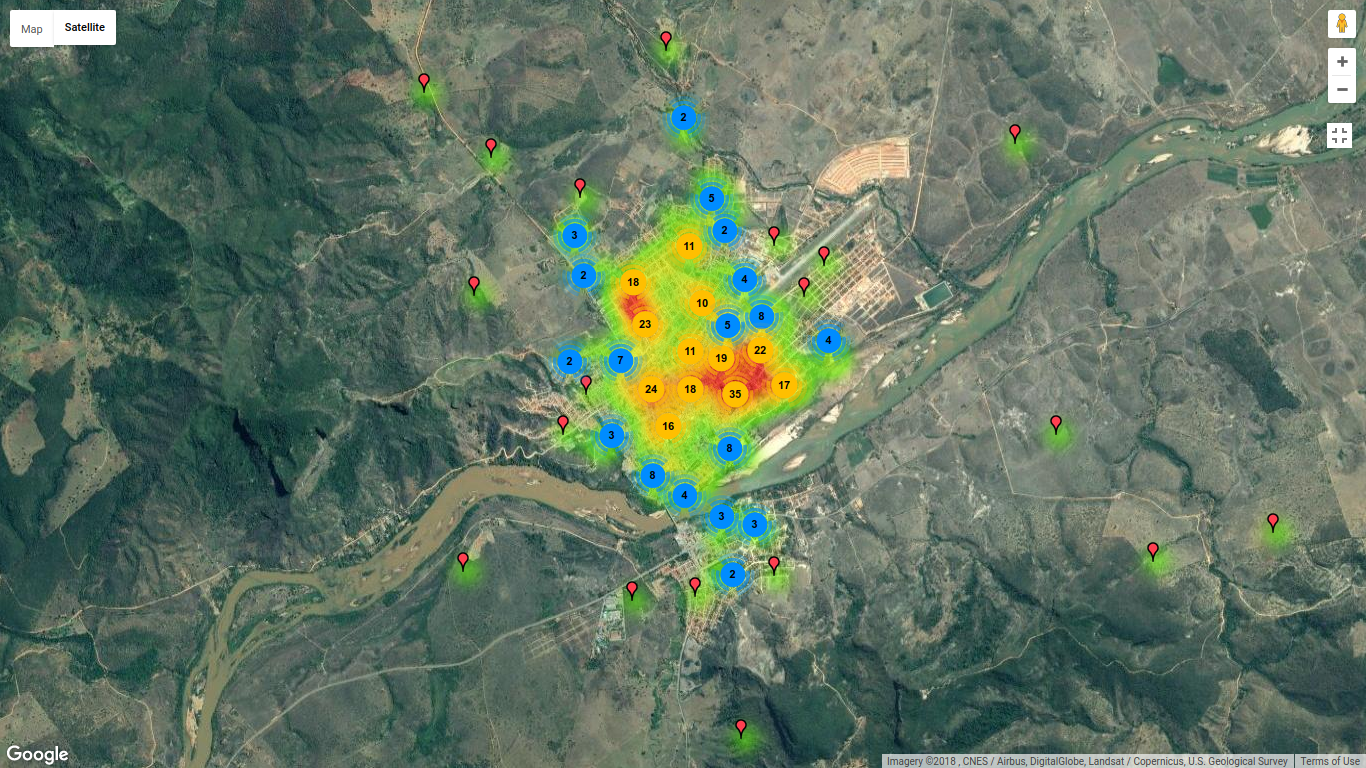
\includegraphics[width=0.6\linewidth]{Imagens/03}
	\legend{Fonte:\url{http://www.cidadaodovale.xyz/inicio.php}}
\end{figure}

% VIAS PÚBLICAS
\begin{figure}[H]
	\centering
	\caption{Densidade Kernel das contribuições sobre problemas nas vias públicas.}	
	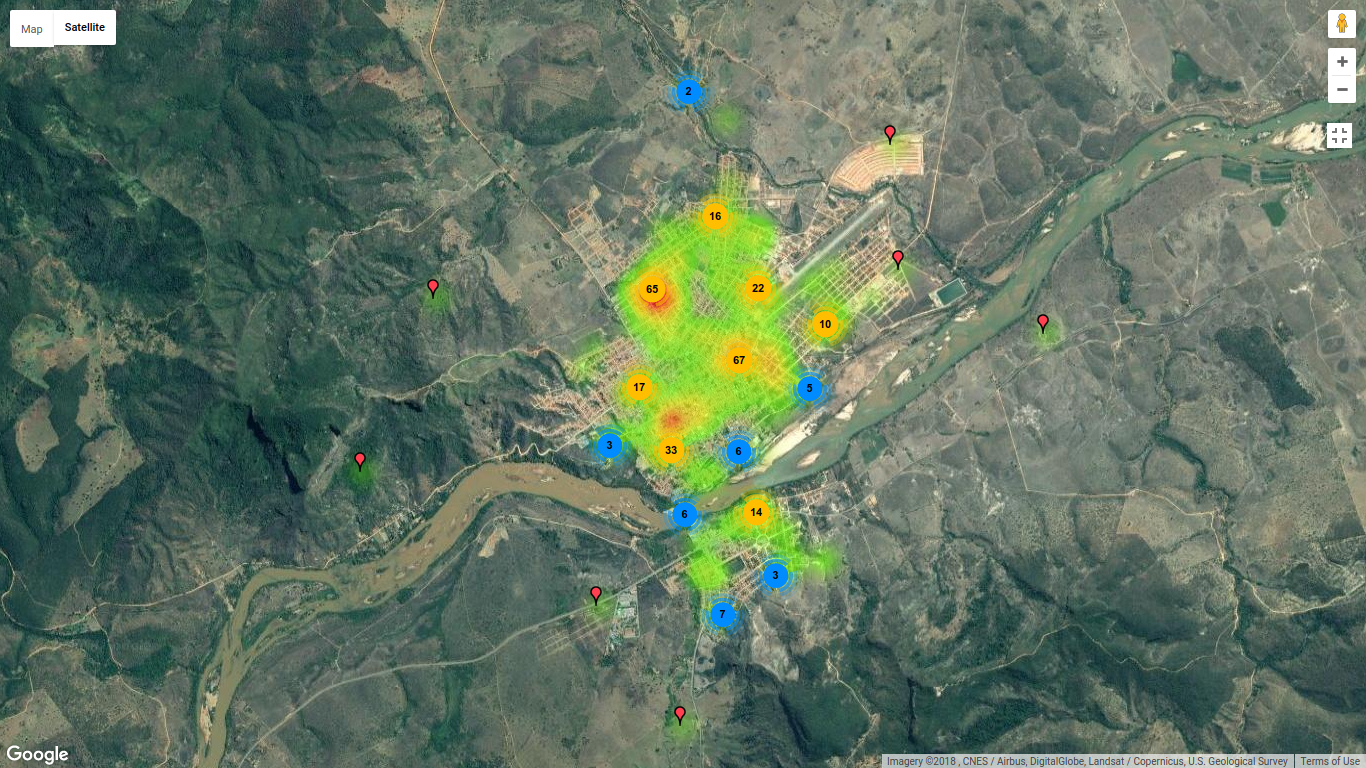
\includegraphics[width=0.6\linewidth]{Imagens/04}
	\legend{Fonte:\url{http://www.cidadaodovale.xyz/inicio.php}}
\end{figure}

\section{Cordova}
Conforme apresentado na documentação oficial \citeonline{the_apache_software_foundation_architectural_nodate} o Cordova é um framework de código aberto que permite a utilização de linguagens padrão da web para o desenvolvimento de aplicativos multiplataformas. Ele utiliza as linguagens padrão da web, HTML5\footnote{Hypertext Markup Language – linguagem de marcação de hipertexto.}, CSS3\footnote{Cascading Style Sheets – estilo de folha em cascata.}, e JavaScript.

\citeonline[p.~2]{lopes_sergio_aplicacao_2016} afirma que, o Cordova é responsável por criar uma "casca nativa" para o aplicativo, na qual gera uma janela de navegador, que faz comunicação entre as chamadas de código para chamadas nativas quando necessário. A Figura 7 mostra a arquitetura do Cordova, na qual utiliza de APIs para realizar a comunicação entre o sistema e o a web, possibilitando assim o acesso a funcionalidades de qualquer aparelho, como sensores, dados, status da rede etc . 

\begin{figure}[H]
	\centering
	\caption{Arquitetura do Cordova}	Cordova cria uma "casca nativa" para o aplicativo 
	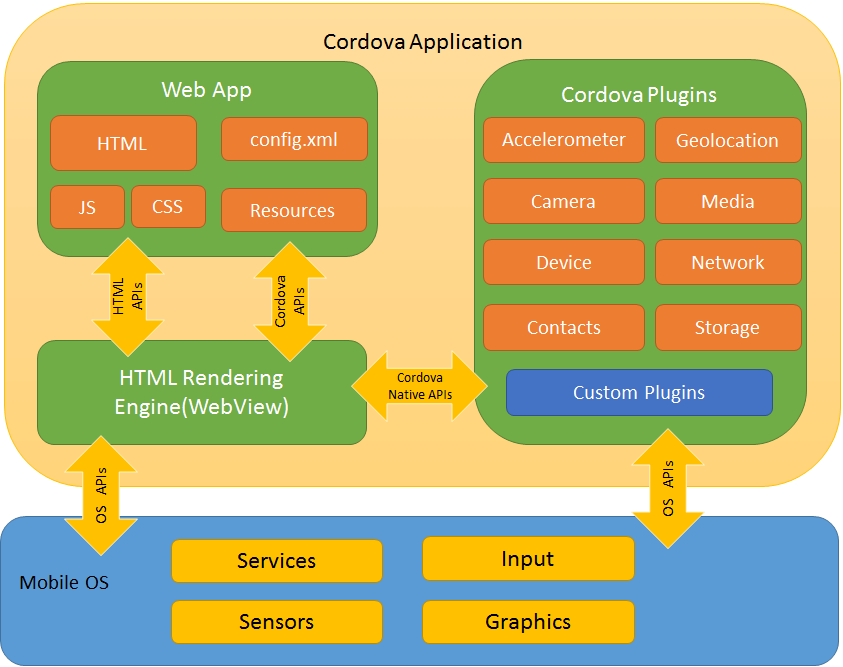
\includegraphics[width=0.6\linewidth]{Imagens/cordovaapparchitecture.png}
	\legend{Fonte:\url{https://cordova.apache.org/docs/en/latest/guide/overview/index.html}}
\end{figure}

\section{Firebase}
O Firebase é um sistema online desenvolvido pela Google do qual possui vários serviços, como banco de dados em tempo real, acesso offiline, aramaz
\citeonline{khawas_application_2018} afirma que o Firebase é uma plataforma online, que auxilia os de desenvolvedores a criarem aplicações de qualidade, ele trabalha com armazenamento NoSQL, no qual realiza os armazenamentos em formato JSON\footnote{JavaScript Object Notation - Objeto de notação JavaScript}, pela Google, que possui vários serviços para diversas plataformas. Segundo \citeonline{silva_junior_and_buregio_vanilson_2016} o Firebase possui uma sincronização em tempo real para Android, iOS e JavaScript, que possibilita o aplicativo esteja responsivo e funcionando offline.
